\documentclass[twocolumn,10pt]{article}
\usepackage[a4paper, top=1.0in, bottom=1.0in, left=0.85in, right=0.85in]{geometry}

\usepackage{graphicx}
\usepackage{algorithm}  
\usepackage{algorithmicx}  
\usepackage{algpseudocode}  
\usepackage{amsmath}

\renewcommand{\algorithmicrequire}{\textbf{Input:}}  
\renewcommand{\algorithmicensure}{\textbf{Output:}}  
\graphicspath{{figure/}}

\begin{document}

%don't want date printed
\date{}

%make title bold and 14 pt font (Latex default is non-bold, 16 pt)
\title{\bf Grouper: A Group Finance Manager on Mobile devices Using Untrusted Servers}

\author{Department of Computer Science
	\\ Meng Li 201620728  
	\\ Supervisor: Yasushi Shinjo
	\\ November 17th, 2016
}

\maketitle

\section{Introduction}
Conventional mobile applications are based on a client-server mode, which requires a central server for storing shared data. This means the users of the mobile applications must fully trust central servers and their application providers. Once a server is attacked by hackers, user information may be revealed because data is stored on only one server with cleartext. Finally, users may lose their data when service providers shut down their services.

Thus, we are going to implement a group finance manager application, Grouper, which is not relied on central servers. This means user data cannot be cracked easily and its service can be recovered after shutting down the old service. Recently, most popular way is using P2P(Peer to Peer) to transfer user data between devices. However, there is a obvious problem in such a no-server proposal. Data transfer can only be finished during two devices is online in a same time. Another problem is that the number of P2P connections will be increased fast as the number of users in a increases because each device can create  connections to all of the other devices. 

To address this problem without using P2P, we use multiple untrusted servers for synchronization. Data will divided to several pieces and uploaded to diverse servers. Each server can only save a piece of data temporarily, which means this piece will be deleted after a period time we specified. Those two rules explained above can ensure that user data cannot be cracked easily. In fact, we can regard untrusted servers as bridges between devices of group members. In addition, all devices of group members have saved a complete data set, data can be recovered even untrusted servers shut down. By this way, we think such a method can satisfy the requirements for an application which is running on untrusted servers, and not relied on central servers.

\section{Methodology}

We implement such a group finance manager application, Grouper, on mobile devices, which is not relied on central servers. 

\subsection{Group Finance Manager}
The goal of a group finance manager is to develop an application that can record the income and expenditure of a small group. In Grouper, group members can create a record including money, classification, account, shop, remark and time. With data synchronization, group members can share their record with other group members, so that group income and expenditure information can be analyzed and shown to all members. Grouper using multiple untrusted servers to synchronize, can avoid defects of applications relied on central servers. 

\subsection{Synchronize with Multiple Untrusted Servers}

We implement Grouper based on data synchronization by multiple untrusted servers rather than a single server. There are three principles in our proposal. 

Firstly, data transfer by a server, but data does not save on this server permanently. Most current popular client-server applications store user data on several central servers, user data will not be deleted unless user deletes his account. Grouper use untrusted servers as a bridge for transferring data. Consider that a group include three members: Alice, Bob and Carol. Alice created a new record in her device, this record will be upload to untrusted servers, and the record on servers will eliminated after Bob and Carol synchronized it from servers. In other words, untrusted servers stores a record until it is be synchronized by all group members.

Secondly, server keep data temporarily. We define a period of time in which data can be saved in a server. In this paper, we set this period to 1 hour for our example situations. This means the record Alice uploaded to untrusted servers can only exist for 1 hour. After 1 hour since uploaded, this record will be deleted. Alice is required to resend this record to serves until all of other members has synchronized successfully. However, the longer keeping period means the higher risk of data reveal. The most suitable period is influenced by the number of group members, security requirement, user expectations and others. 

Thirdly, servers do not know the content of data. Saving data temporarily cannot ensure data security, because servers know the cleartext of data in this temporary period. For this problem, developers often encrypt data before uploading to servers, which need a private key to decrypt data in other devices. In order to distribute the private key, users should share it by themselves. In this paper, we use secret sharing, which can create a number of shares and distributing them to a set of participants\cite{smith2013layered}, to share data between user devices and untrusted servers.

\begin{figure}[t]
\centering
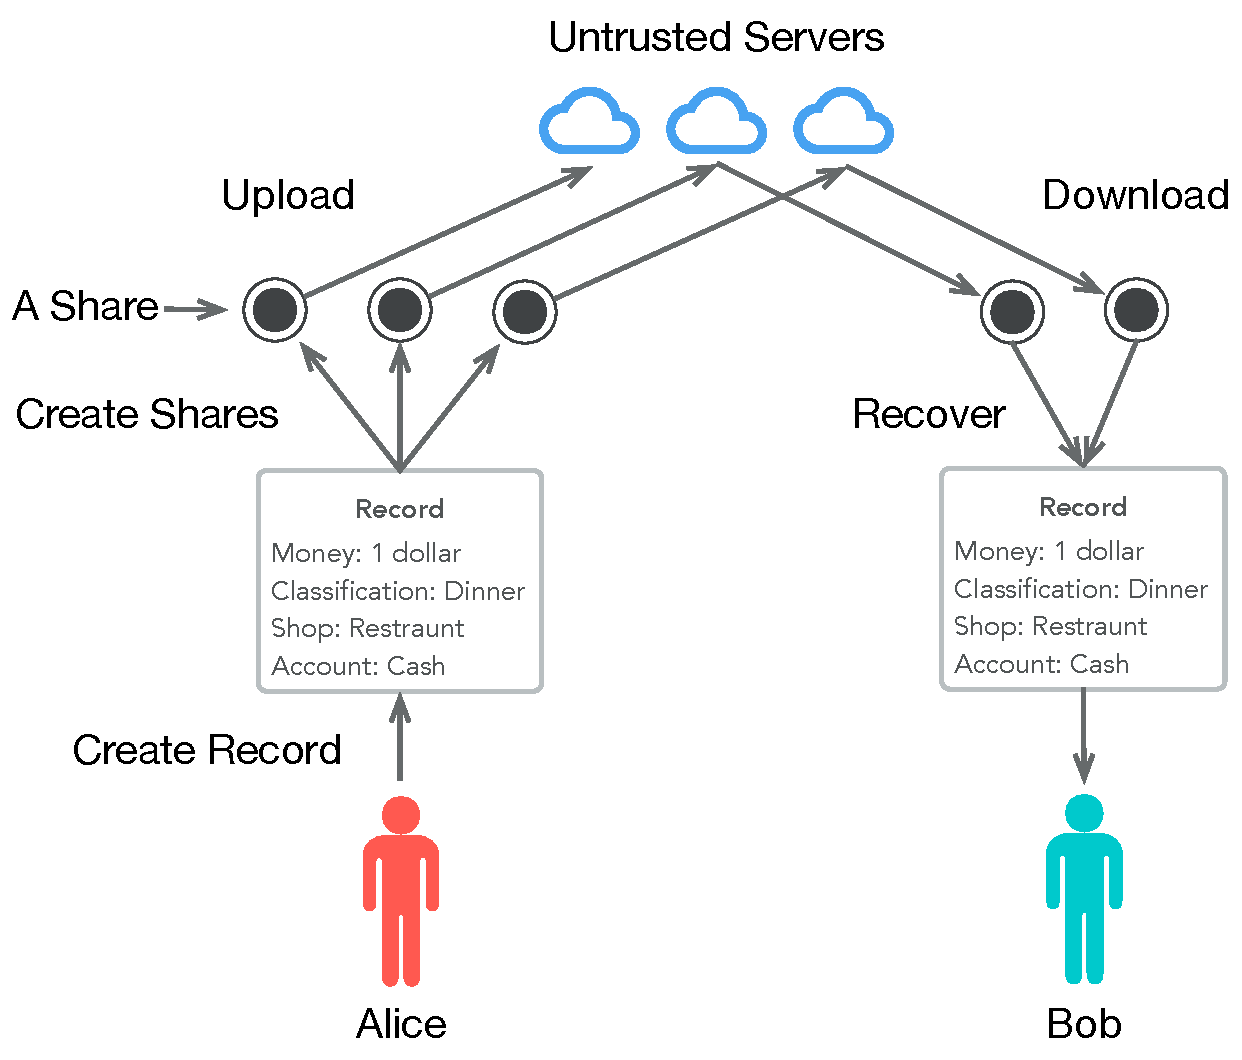
\includegraphics[scale=0.4]{sync_flow}
\caption{Flow of Synchronization}
\end{figure}
Based on the three core principles introduced above, our synchronization flow can be described as Figure 1. At first, Alice add a record and Grouper creates a number of shares by secret sharing. Then, Grouper uploads those shares to multiple untrusted servers. When Bob is online, Grouper in Bob's device will download shares from servers and recover the new record uploaded by Alice. In this situation, Grouper can recover the record after getting more than two shares. In this process, each server is separated from other servers, and cannot access to other servers. This means user data can not be recovered unless you have permission access to more than two servers. In our proposal, only group members have permission to access these untrusted servers.

\subsection{Shamir's Secret Sharing}
Secret sharing which can create a numbers of shares, plays an indispensable role in protecting user data from getting lost, destroyed, or into wrong hands. In this paper, we use Shamir's secret sharing, a form of secret sharing proposed by Shamir and Blakley independently. In a secret sharing scheme, a dealer securely shares a secret with a group of participants, by generating $n$ shares using a cryptographic function\cite{smith2013layered}. At least $k$ or more participants can reconstruct the secret, but $k-1$ or fewer participants can obtain nothing about the secret\cite{pang2005new}. We describe this scheme as a function $f(k, n)$, where n is the number of all shares, and k is the threshold to combine shares. A popular technique to implement threshold schemes uses polynomial interpolation ("Lagrange interpolation"). This method was invented by Shamir in 1979. Thus, we call it Shamir's Secret Sharing.

There are many implementations of Shamir's secret sharing by different programming languages. For developing an iOS app by Objective-C, we need an implementation without limitation of length, which supports Objective-C language and UTF-8 character set. c-SSS\cite{c-sss} is an implementation in original C code of Shamir's Secret Sharing by Fletcher T. Penney. c-SSS provide two main functions for generate shares and reconstructing them. Function \emph{generate} can generate $n$ shares by the string text with the threshold $k$. Function \emph{extract} can recreate the text string after accessing to more than $k$ shares.

\subsection{Reliable Synchronization}
Grouper should provide a reliable synchronization service. For example, once Alice, who is a user in a group, creates a new record in her device, all of other members in a group should synchronize this record, even if this record may be deleted by untrusted servers after 1 hour. We call this problem \emph{Reliable Synchronization}.

\begin{figure}[t]
\centering
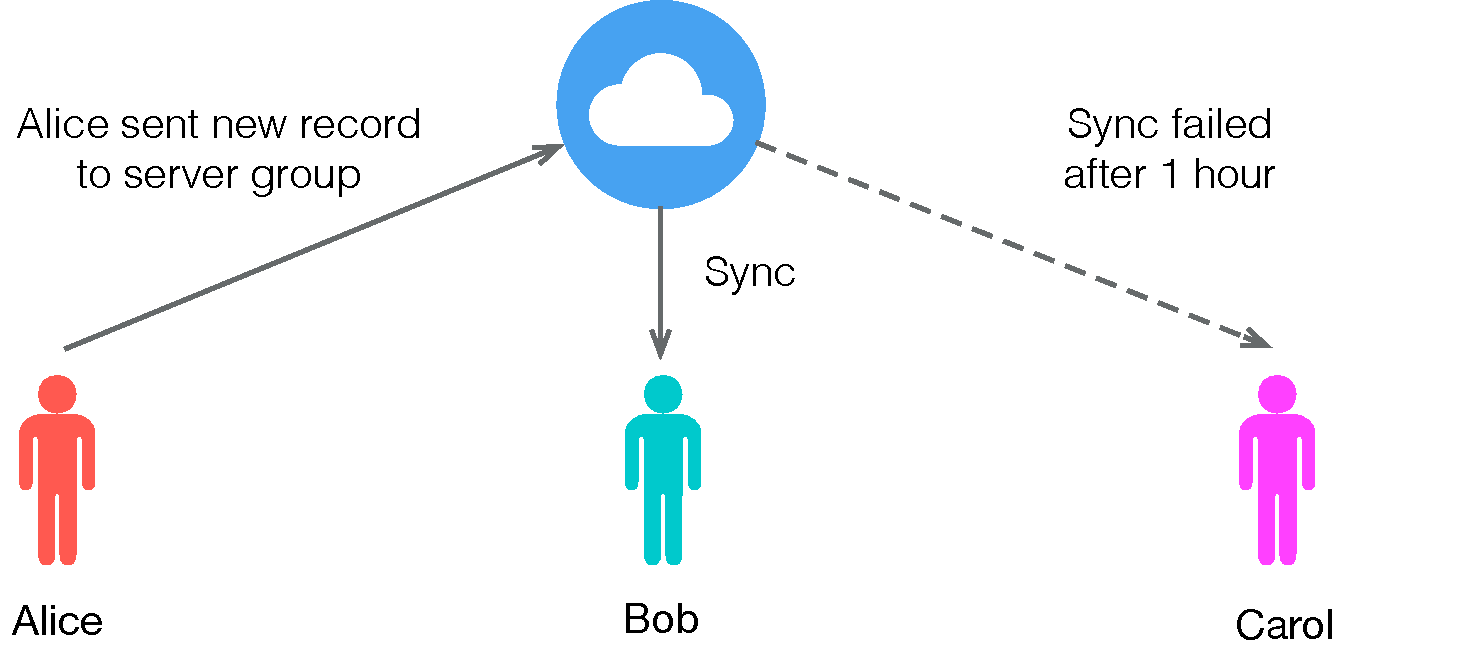
\includegraphics[scale=0.4]{sync_completely}
\caption{Sync Completely}
\end{figure}

Figure 2 describes the situation data cannot be synchronized completely. Alice sent a new record to untrusted servers in 10:00 AM and Bob synchronized it successfully before 11:00 AM. Carol forgot to synchronize this record before 11:00 AM. She cannot synchronize after 11:00 AM because servers has delete the record in 11:00 AM. To solve this problem, Alice resend her new record until Carol synchronize it successfully. However, by what way can Alice get the information that all of other members in her group have synchronized. In other words, it is an unreasonable requests for Alice to resend her record indefinitely. It is necessary for us to find an efficient way for notifying Alice that all members have synchronized successfully.

We design a counter in clients as the solution to the \emph{Reliable Synchronization} problem. Intuitively, this counter calculates the number of times other clients synchronized and works on the sender to decide resending record or not. The condition that sender device needs not to resend a record can be described as equation 1.
\begin{equation}
\sum_{i=1}^{n}s_{i}=(m-1)\cdot k
\end{equation}

In Equation 1, we suppose that there are $n$ untrusted servers, Server 1, Server 2,..., Server $n$. We can also look at $n$ from a different perspective. This is the first parameter, the number of all shares, in the scheme $f(k, n)$ of Shamir's secret sharing. Each server saves a share, so $n$ servers saves $n$ shares. Each server should know how many times the share has been downloaded by clients. Thus, we use $s_i$ to represent the number of download times in server $i$. The sum of $s_i$ is calculated in the sender client. In the left of equation 1, $m$ represents the number of group members, and $k$ is the threshold in scheme $f(k, n)$. Obviously, a client can reconstruct data after getting $k$ shares. If $m-1$ clients have reconstructed data, $(m-1)\cdot k$ shares is downloaded. That means clients except sender has synchronized successfully, so the sender need not to resend.

To implement such a counter, restriction about security and connection should be considered. Remember that servers cannot communicate with each other. Actually, one server of the group does not know the others in the group. On the other hand, clients cannot communicate with each other. Clients do know IP address or domain name of other device, so that they cannot send messages with P2P connections. We design sender table in clients and transfer table in servers described as Figure 3 to address this problem. 

\begin{table}[tbp]
	\centering  
	\begin{tabular}{lll}  
		\hline
		Column &Data Type & Introduction\\ 
		\hline  
		sid &String & Physical unique identifier\\
		content & String & JSON String of object\\ 
		object & String & Name of object\\
		count & Integer16 & Count of sync time\\
		resend & Boolean &Necessity of resending data \\
		sendtime & Date & Data send time\\
		\hline
	\end{tabular}
	\caption{Columns of sender table}
\end{table}

Columns of a sender table is listed in table 1. Here, sid, content, and count of sync times are main columns. Sid is an unique identifier created by SQLite database in client, it is same as those in servers; content saves the JSON string converted by new record object; count saves the sync times of this object. In server, transfer table also has these 3 main columns with different meaning. Sid is equals to which in client in order to point out the row corresponding to which in client; content saves one of the shares generated by secret sharing scheme; count saves the content sync times in server. Other auxiliary columns in transfer table will not be introduced here.
Suppose the secret sharing scheme is $f(2, 3)$, and only Bob have synchronized Alice's new record within prescribed time-limit. In figure 3, the column corresponding to Alice's new record, whose id is 1, is equals to those columns whose ids are 1 in server 1 and server 2. This is to say Bob downloaded two shares from server 1 and server 2. Client of Alice will know that by HTTP response from server 1 and server 2 when it resend data. It will send for one more time, because it's count is 2, which is less than 4, the threshold Alice need not resend.

\begin{figure}[t]
\centering
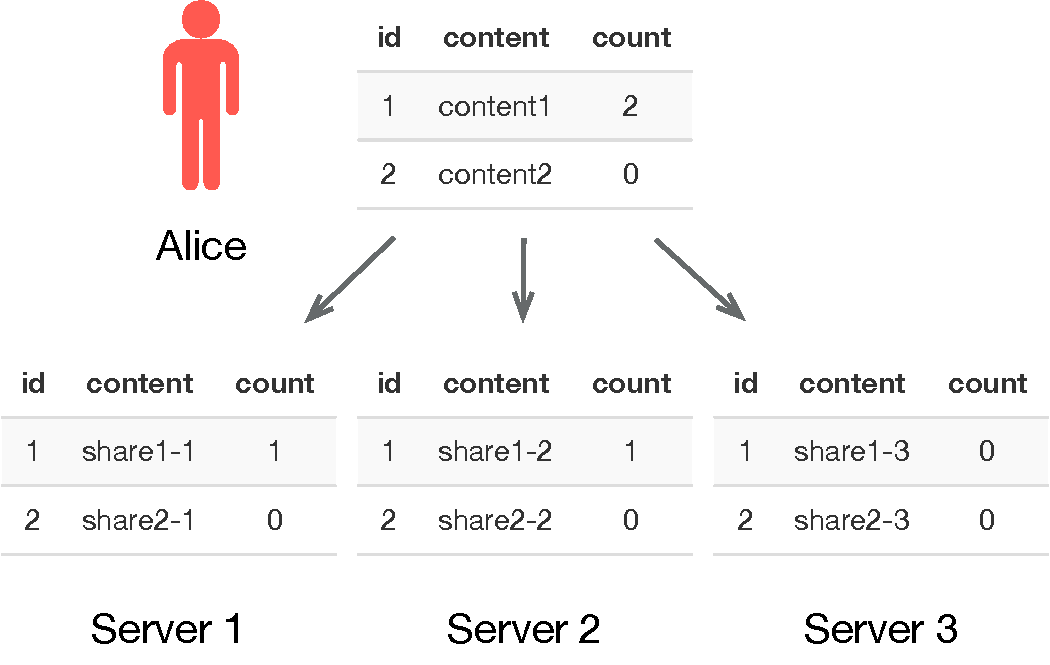
\includegraphics[scale=0.4]{sync_table}
\caption{Sync Table}
\end{figure}

\section{Architecture}
Grouper consists of an iOS app for clients and a Web service in servers.

\subsection{Architecture in Client}
In Methodology, we have introduced how to sharing a string with other deices via multiple untrusted servers. In this section, we about persistent store and data synchronization. With untrusted servers, Grouper have to store all data on mobile devices with an object-oriented way. Grouper use Core Data\cite{coredata}, a native iOS framework to manage the model layer objects. Core Data provides generalized and automated solutions to common tasks associated with object life cycle and object graph management, including persistence, to store and operate data as object. Sync\cite{sync} by Elvis Nuñez, a modern Swift JSON synchronization framework to Core Data, can help we implement data synchronization easily in Grouper by parsing a JSON response and getting it into Core Data. With Sync based on Core Date, we can concentrate on sharing with untrusted servers rather than data storage and synchronization.

c-SSS by Fletcher T. Penney can generate shares from a JSON string saved on a sender table. Grouper is developed with Objective-C language, which is compatible with original C code. Grouper generates shares and send them by a REST API to servers until this record needs not to resend.

\begin{figure}[t]
\centering
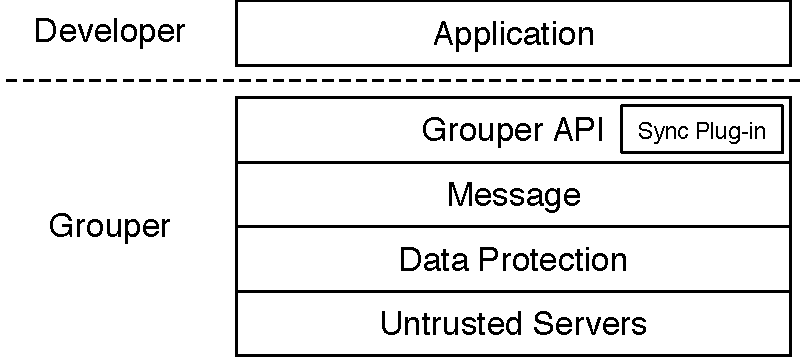
\includegraphics[scale=0.4]{architecture}
\caption{Architecture}
\end{figure}

\subsection{Web Sync Gate}
Many applications with synchronization is based on commercial cloud services like Amazon S3, Google Cloud or iCloud. It is necessary that Grouper has its own web service running on individual server rather than using commercial cloud services directely for following reasons:

\begin{itemize}
\setlength{\itemsep}{1pt}
\setlength{\parskip}{0pt}
\setlength{\parsep}{0pt}
    \item Data Storage: untrusted servers save share generated by secret sharing.
    \item Provisionality: web service ensure that share will be delete within prescriptive time.
    \item Security: only group members who has access key can download share from server. In other word, web service plays a role of access control.
    \item Counter: web service palys a role of counter to calculate sync times in server.
\end{itemize}

\section{Related Work}

DepSky\cite{bessani2013depsky} is a system that storage encrypted data on servers and run application logic on the client-side\cite{wang2016sieve}. DepSky provide a storage service that improves the availability and confidentiality provided by commercial storage cloud services. \emph{Cloud-of-Clouds} is the core concept in DepSky. It represents that DepSky is a virtual storage cloud, which is accessed by its users by invoking operations in several individual severs. DepSky saves encrypted data in commercial storage cloud services and do application logic in individual servers. In Grouper,  untrusted servers undertake responsibility of temporarily data storage and message delivery with server-side computation. Thus, Grouper cannot only use commercial storage cloud services.

Mylar\cite{popa2014building} stores sensitive data encrypted on the server, and decrypts that data only in users’ browsers. Developer should uses Mylar’s API to encrypt a regular (non-encrypted) web application, and users decrypt data by browser extension. Like Grouper, application in Mylar can control how user data is shared\cite{wang2016sieve}; unlike Grouper, Mylar build its system on a browser with browser extension while Grouper use mobile devices as client.

Of course, there are many applications or frameworks synchronize with untrusted network and servers. Compared to them, Grouper use secret sharing and temporary data storage with untrusted servers to protect user data from malicious attacking.

\section{Future Work}

An application running in client has been developed now. In future, we are going to develop a web service running on multiple untrusted servers to manage data temporary storage and provide REST API for mobile devices. This web service developed by Java EE should be install by group owner, in order that nobody except the group owner know all the IP address of servers. Thus, security of Grouper can be guaranteed.

\section{Conclusion}

This paper introduced Grouper, a group finance manager, using secret sharing and data synchronization on mobile devices. Grouper is synchronized by multiple untrusted servers, each server of which does not know existence of others. Each server only saves one of the shares generated by secret sharing temporarily, to ensure that user data cannot be cracked easily.

\bibliographystyle{unsrt}
\bibliography{ref}

\end{document}
